% Generated by scripts/txt2tex.py from chapters/chapter_05.txt. Edit the TXT, not this file.
\chapterlayout{05}
\chapterquestion{איך יודעים שמכונה באמת למדה, ולא רק נשמעת כאילו למדה?}
\chapter{בודקים מודלים בעזרת נתונים}\label{ch:05}
\section{השאלה שאחרי התשובה}
התשובה על הבצק כבר ממלאת את המסך. היא מסודרת בסעיפים, מנוסחת בביטחון, ואפילו מציעה מה לעשות עכשיו. אבל אחרי הקריאה הראשונה הקוראת נעצרת מול שאלה שקטה יותר: איך אני יודעת שזה נכון? ומי בדק את המערכת הזאת לפני שהגיעה אליי?
את מודל השפה שענה לה הספר לא יכול לפרק ולבחון. אבל אפשר להראות מקרוב את העיקרון שעליו נשענת בדיקה של מערכת לומדת: לא שואלים אותה על מה שכבר ראתה. מודל טוב הוא מודל שמנבא היטב גם על נתונים חדשים, ולתכונה הזאת קוראים הכללה (generalization) \cite{S-ch05-08}. כדי למדוד אותה מציבים מול המכונה דוגמאות שלא פגשה מעולם, ומונים כמה פעמים צדקה.
וזה מה שנעשה בפרק הזה, ובסופו הספר יריץ ניסוי משלו.
\section{לספור פגיעות}
המדד הפשוט ביותר נקרא דיוק (accuracy): החלק היחסי של התחזיות שתואמות את התשובה האמיתית \cite{S-ch05-01}. התיעוד של ספריית scikit-learn מביא דוגמה זעירה: ארבע דוגמאות שהתוויות האמיתיות שלהן הן 0, 1, 2 ו-3, ומודל שעונה 0, 2, 1 ו-3. שתי תשובות נכונות מתוך ארבע, כלומר דיוק של 0.5 \cite{S-ch05-01}.
\begin{conceptbox}{דיוק ושיעור שגיאה}
בפרק 1 פגשנו מסנן דואר זבל, ואת מדד הביצוע שלו: החלק של ההודעות שסווגו נכון. למדד הזה יש שם. כל הודעה מסתיימת באחת מארבע תוצאות: זבל שהגיע לתיקיית הזבל (חיובי אמיתי, TP), הודעה תקינה שנשלחה לשם בטעות (חיובי שגוי, FP), זבל שחמק לתיבה הנכנסת (שלילי שגוי, FN), והודעה תקינה שהגיעה למקומה (שלילי אמיתי, TN) \cite{S-ch05-07}.
\begin{equation}
\text{Accuracy} = \frac{TP + TN}{TP + TN + FP + FN}
\end{equation}
במונה: שתי ההחלטות הנכונות. במכנה: כל ההודעות \cite{S-ch05-06}.
שיעור השגיאה (error rate) הוא המשלים: שיעור השגיאה = 1 פחות הדיוק.
\end{conceptbox}
מספר אחד נוח לזכור, אבל הוא גם נוח להסתיר. חומרי הלימוד של Google מציגים מקרה מאלף: אם מחלקה מסוימת מופיעה רק באחוז אחד מהמקרים, מודל שעונה תמיד "לא" יקבל דיוק של 99\%, ובכל זאת אין בו שום תועלת \cite{S-ch05-06}. כשהנתונים לא מאוזנים, או כשסוג אחד של טעות יקר מהשני, עדיף להיעזר במדדים שמסתכלים על כל סוג טעות בנפרד \cite{S-ch05-06}.
\section{שני סוגים של טעות}
שני מדדים כאלה שווה להכיר בשמם. הראשון הוא דייקנות (precision): מתוך כל מה שהמסווג סימן כחיובי, כמה היה חיובי באמת. לפי תיעוד scikit-learn, זו היכולת שלו לא לתייג דוגמה שלילית כחיובית \cite{S-ch05-01}. השני הוא כיסוי (recall): מתוך כל הדוגמאות החיוביות שהיו שם, כמה הוא הצליח למצוא \cite{S-ch05-01}. בשפת ארבע התוצאות, הדייקנות היא TP חלקי סכום TP ו-FP, והכיסוי הוא TP חלקי סכום TP ו-FN \cite{S-ch05-06}. במסנן הדואר, דייקנות נמוכה פירושה הודעות תקינות שנבלעות בתיקיית הזבל, וכיסוי נמוך פירושו זבל שממשיך להציף את התיבה.
אותו תיעוד מביא דוגמה קטנה שאפשר לחשב ביד: שמונה דוגמאות, שלוש שליליות וחמש חיוביות. מתוך שלוש השליליות המסווג זיהה נכון שתיים וטעה באחת (TN=2, FP=1), ומתוך חמש החיוביות מצא שלוש והחמיץ שתיים (TP=3, FN=2) \cite{S-ch05-01}. הדיוק הוא 5 מתוך 8, כלומר 0.625, ושיעור השגיאה 0.375. הדייקנות היא 3 מתוך 4, כלומר 0.75, והכיסוי 3 מתוך 5, כלומר 0.6.
\begin{table}[htbp]
\centering
\caption{מדדים במבט אחד}\label{tab:5.1}
\begingroup\small\renewcommand{\arraystretch}{1.35}\booktablerule
\begin{tabularx}{\linewidth}{RRRR}
\toprule
\rowcolor{midnight}\tabhead{מדד} & \tabhead{השאלה שהוא עונה עליה} & \tabhead{נוסחה} & \tabhead{מה נעלם ממנו}\\ \midrule
דיוק (accuracy) & באיזה חלק מכל המקרים המודל צדק? & (TP+TN) / (TP+TN+FP+FN) \cite{S-ch05-06} & כשמחלקה נדירה, גם מודל חסר תועלת מציג דיוק גבוה \cite{S-ch05-06}\\
שיעור שגיאה (error rate) & באיזה חלק מהמקרים המודל טעה? & 1 פחות הדיוק (נגזר מהנוסחה) & אותה חולשה כמו הדיוק, כי זה אותו מידע בהיפוך\\
דייקנות (precision) & מתוך מה שסומן כחיובי, כמה חיובי באמת? & TP / (TP+FP) \cite{S-ch05-06} & החיוביים שהוחמצו: הנוסחה אינה כוללת את FN\\
כיסוי (recall) & מתוך החיוביים שהיו, כמה נמצאו? & TP / (TP+FN) \cite{S-ch05-06} & התרעות השווא: הנוסחה אינה כוללת את FP\\
\bottomrule
\end{tabularx}
\endgroup
\end{table}
התיעוד של scikit-learn מציע גם דיוק מאוזן (balanced accuracy), שנועד למנוע הערכות מנופחות כשהמחלקות אינן מאוזנות \cite{S-ch05-01}. וסוקולובה ולפאלם (Sokolova \& Lapalme) פרסמו ב-2009 ניתוח שיטתי של מדדי ביצוע למשימות סיווג \cite{S-ch05-11}.
כאן מתחילה הערכת תוצאות (evaluation), שהיא יותר מחישוב של מספר. היא פותחת בשאלה על אילו נתונים נמדד המספר, ממשיכה בשאלה איזו טעות יקרה יותר במשימה הזאת \cite{S-ch05-06}, ורק אז בוחרת מדד. דמיינו מי שמחכה למכתב חשוב: היא תעדיף שקצת זבל יחמוק לתיבה, ובלבד שהמכתב לא ייעלם בתיקיית הזבל. בשבילה, דייקנות חשובה יותר מכיסוי. והשאלה האחרונה אינה פחות חשובה: מה המספר עלול להסתיר.
\section{שתי ערמות של דוגמאות}
נניח שמודל למד לזהות ספרות בכתב יד. אם נמדוד את הדיוק שלו על אותן דוגמאות שמהן למד, נקבל דיוק אימון. אם נמדוד על דוגמאות שהוחזקו בצד, נקבל דיוק בדיקה. רק הוא מספר משהו על ההכללה. זו החלוקה לאימון ולבדיקה שפגשנו בפרק 2. השגיאה על הדוגמאות שבצד היא אומדן של מה שבאמת מעניין אותנו: השגיאה הצפויה של המודל על נתונים חדשים \cite{S-ch05-13}. להפרש בין השגיאה הזאת לשגיאת האימון קוראים פער הכללה (generalization gap) \cite{S-ch05-12}. יש חוקרים שמכנים את הפער הזה גם שגיאת הכללה (generalization error) \cite{S-ch05-10,S-ch05-12}.
דמיינו קורא כתב יד שלא למד את צורת הספרה 4, אלא שינן כל כתם דיו וכל רעד של עט בערמה שהוצגה לו. על הערמה הזאת הוא כמעט לא טועה. כשמגיעה מעטפה מכותב חדש, הוא אובד עצות. לתופעה הזאת קוראים התאמת יתר (overfitting): מודל שתואם את קבוצת האימון (משנן אותה) עד כדי כך שהוא נכשל בחיזוי נכון על נתונים חדשים. הכללה היא ההפך שלה. ובתת-התאמה (underfitting) המודל אינו מנבא טוב אפילו על נתוני האימון \cite{S-ch05-08}.
תיעוד scikit-learn מציע כלל אצבע לקריאת עקומות, שמשווה בין ציון האימון לבין הציון על קבוצת אימות (validation set), כלומר נתונים שהמודל לא למד מהם. אם שני הציונים נמוכים, זה סימן לתת-התאמה: המודל פשוט מדי ולא תפס את הדפוס. אם ציון האימון גבוה וציון האימות נמוך, זה סימן להתאמת יתר. ומצב הפוך, ציון אימון נמוך עם ציון אימות גבוה, בדרך כלל אינו אפשרי \cite{S-ch05-02}. (בניסוי של הספר אין קבוצת אימות; ציון הבדיקה שבו משמש לדיווח בלבד.)
\begin{mythbox}
\mythlabel מודל שמגיע לדיוק כמעט מושלם על נתוני האימון הוא מודל טוב.
\tcblower
\realitylabel במאמר שהוצג בכנס ICLR ב-2017 הראו ג'אנג (Zhang) ועמיתיו שרשתות עמוקות מצליחות "ללמוד" גם תוויות שהוגרלו באקראי. שגיאת האימון מגיעה לאפס, ושגיאת הבדיקה אינה טובה מניחוש מקרי \cite{S-ch05-10}. במערך התמונות CIFAR10, מודל Inception שאומן על תוויות אקראיות הגיע ל-100.0\% דיוק אימון ול-9.78\% בלבד בבדיקה (טבלה 1 במאמר) \cite{S-ch05-10}. התמונות עצמן היו אמיתיות, אבל בינן לבין התוויות לא היה שום קשר. ובכל זאת הרשת שיננה כל אחת מהן, ורק קבוצת בדיקה נפרדת חשפה זאת.
\end{mythbox}
\section{הניסוי של הספר: ספרות בכתב יד}
בפרק 1 פגשנו את המכונות שממיינות דואר לפי ספרות שנכתבו ביד. עכשיו הספר מריץ בעצמו מודל קטן על ספרות בכתב יד, ומודד אותו כפי שתואר כאן.
הנתונים מגיעים מהמאגר שנקרא Optical Recognition of Handwritten Digits, של אלפיידין וקיינק (Alpaydin \& Kaynak), שנתרם ב-1998 למאגר UCI Machine Learning Repository ומופץ ברישיון פתוח CC BY 4.0 \cite{S-ch05-05}. המאגר המלא כולל 5,620 דוגמאות \cite{S-ch05-05}. הניסוי משתמש בעותק שמופץ עם scikit-learn תחת השם load\_digits: 1,797 תמונות של ספרות, כל אחת רשת של 8 על 8 משבצות, כלומר 64 תכונות, שבכל אחת מספר שלם בין 0 ל-16, ועשר מחלקות, הספרות 0 עד 9 \cite{S-ch05-04}. לפי התיעוד, זה עותק של קבוצת הבדיקה של המאגר המקורי \cite{S-ch05-04}.
\begin{labbox}{איך נבנה הניסוי}
\begin{enumerate}
\item טוענים את 1,797 הספרות \cite{S-ch05-04}.
\item מחלקים אותן פעם אחת: 75\% לאימון ו-25\% לבדיקה, בחלוקה מרובדת לפי ספרה. יוצאות 1,347 דוגמאות אימון ו-450 דוגמאות בדיקה. זרע אקראי (seed) קבוע, 42, מבטיח שכל הרצה חוזרת תיתן את אותה חלוקה.
\item מנרמלים את הערכים, והנרמול נלמד מקבוצת האימון בלבד, כדי שמידע מהבדיקה לא יזלוג פנימה.
\item מאמנים רשת נוירונים קטנה: שכבה חבויה אחת של 32 נוירונים, במשך 40 תקופות אימון (epochs). בסוף כל תקופה מודדים דיוק על שתי הקבוצות. דיוק הבדיקה נמדד לדיווח בלבד, ולא שימש לאימון, לנרמול או לבחירת מודל או תקופה.
\item שומרים את המספרים לקובץ CSV, ומשם מציירים את הגרף ואת הטבלה.
\end{enumerate}
כלל היושר של הניסוי: כל ההגדרות, כולל מספר התקופות, נקבעו לפני ההרצה. מציגים את מה שיצא. אם לא יופיע פער בין אימון לבדיקה, הספר יאמר זאת, ולא ישנה הגדרות עד שתופיע הצורה "הנכונה".
\end{labbox}
\begin{figure}[htbp]
\centering
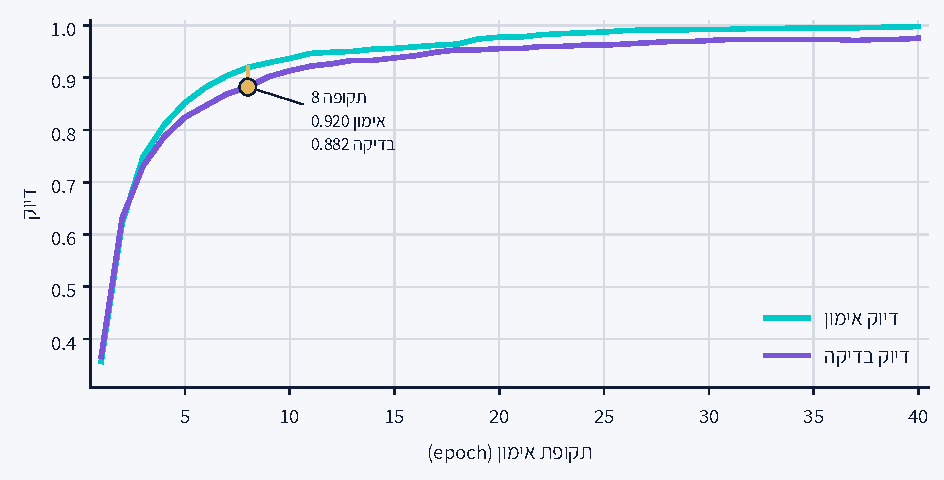
\includegraphics[width=\linewidth]{assets/charts/fig5_1_accuracy.pdf}
\caption{דיוק אימון מול דיוק בדיקה לאורך תקופות האימון}\label{fig:5.1}
\figurenote{המספרים חושבו בניסוי של הספר על נתוני UCI Digits (Alpaydin \& Kaynak, 1998, CC BY 4.0) · מקור: ניסוי M4, python/data/digits\_accuracy.csv שמופק על ידי python/generate\_chart.py}
\end{figure}
\begin{table}[htbp]
\centering
\caption{דיוק אימון ודיוק בדיקה לפי תקופת אימון (ניסוי הספר, UCI Digits)}\label{tab:5.2}
\begingroup\small\renewcommand{\arraystretch}{1.35}\booktablerule
\begin{tabular}{ccc}
\toprule
\rowcolor{midnight}\tabhead{תקופה} & \tabhead{דיוק אימון} & \tabhead{דיוק בדיקה}\\ \midrule
1 & 0.357 & 0.367\\
5 & 0.852 & 0.824\\
8 & 0.920 & 0.882\\
10 & 0.937 & 0.913\\
15 & 0.956 & 0.938\\
20 & 0.978 & 0.956\\
25 & 0.987 & 0.962\\
30 & 0.993 & 0.971\\
35 & 0.995 & 0.973\\
40 & 0.998 & 0.976\\
\bottomrule
\end{tabular}
\endgroup
\end{table}
\section{איך לקרוא את הגרף, ומה לא לקרוא בו}
אפשר לקרוא את הגרף לפי כלל האצבע, אם משאילים אותו מקבוצת אימות לקו הבדיקה (הכלל עצמו מנוסח בתיעוד לקבוצת אימות). אם שני הקווים עולים ונשארים קרובים זה לזה, המודל מכליל היטב על החלוקה הזאת. אם דיוק האימון גבוה ודיוק הבדיקה נמוך ממנו בהרבה, זה המצב שתיעוד scikit-learn מזהה עם התאמת יתר \cite{S-ch05-02}. ואם שני הקווים נשארים נמוכים, זה סימן לתת-התאמה \cite{S-ch05-02}.
יש גרפים שמציגים הפסד (loss) במקום דיוק: מספר שמודד עד כמה התחזיות רחוקות מהתשובות הנכונות, וככל שהוא נמוך יותר, טוב יותר. בעקומות כאלה הסימן המוכר הוא שהפסד האימון ממשיך לרדת בזמן שההפסד על הנתונים שהוחזקו בצד מתחיל לעלות. לפי Google, דפוס כזה מרמז בחוזקה על התאמת יתר \cite{S-ch05-08}.
מה יצא בפועל, כפי שמופיע באיור~\ref{fig:5.1} ובטבלה~\ref{tab:5.2}? שני הקווים עולים מהר עד התקופה העשירית בערך, ואחר כך מתמתנים. דיוק הבדיקה אינו מתדרדר: מלבד ירידה זעירה אחת בתקופה 37 (מ-0.973 ל-0.971, ובתקופה 38 חזרה ל-0.973) הוא מתייצב סביב 0.97 מתקופה 30. דיוק האימון ממשיך להתקרב ל-1. בסוף האימון דיוק האימון הוא 0.998 ודיוק הבדיקה 0.976, פער הכללה מוערך של 2.2 נקודות אחוז. הפער הגדול ביותר, 3.8 נקודות, היה בתקופה 8 (0.920 מול 0.882), והיא הנקודה המודגשת באיור; נבחרה לפי כלל קבוע ולא בעין. לפי כלל האצבע, זו אינה תת-התאמה, כי שני הציונים גבוהים. יש פער קטן ועקבי בין האימון לבדיקה, אבל לא הדפוס של התאמת יתר, שבו הבדיקה מתדרדרת. כדאי לא להסיק מהמספרים יותר מדי. ראשית, זו חלוקה אחת עם זרע אקראי אחד. חלוקה אחרת עשויה לתת קווים מעט שונים, ולכן הגרף מתאר את הניסוי הזה, לא חוק טבע. שנית, אם נבחר בדיעבד את התקופה "הטובה ביותר" לפי קו הבדיקה, הבדיקה כבר השפיעה על ההחלטה. ג'אנג ועמיתיו מעירים שכדי לטעון בקפדנות שעצירה מוקדמת (early stopping) משפרת הכללה, צריך קבוצת בדיקה מבודדת נוספת \cite{S-ch05-10}. שלישית, חומרי הלימוד של Google מזכירים שעקומות הפסד קשות לא פעם לפרשנות \cite{S-ch05-09}. ורביעית, מסווג קטן של ספרות בגודל 8 על 8 פיקסלים אינו מודל שפה. הניסוי מדגים שיטת בדיקה, ולא מעיד דבר על איכות התשובה שהקוראת קיבלה על הבצק.
\section{בחזרה אל המסך}
הקוראת לא תראה לעולם את קבוצת הבדיקה של המערכת שענתה לה. אבל עכשיו היא יודעת מה לשאול: על אילו נתונים נמדדה המערכת, האם אלה נתונים שלא ראתה, איזו טעות נספרה, ומה המספר מסתיר. בדיקה טובה היא תנאי הכרחי לאמון, אבל לא ערובה מלאה: גם מערכת שנבחנה היטב טועה לפעמים, ולפעמים דווקא בטון הבטוח ביותר. על הגבולות האלה, ועל מה שקורה למה שהקוראת הקלידה, נדבר בפרק 6.
\begin{insightsbox}
\begin{itemize}
\item דיוק עונה על שאלה אחת בלבד: באיזה חלק מהמקרים המודל צדק \cite{S-ch05-01}; שיעור השגיאה הוא פשוט המשלים שלו.
\item מספר גבוה יכול להטעות: כשמחלקה נדירה, גם מודל חסר תועלת יכול להציג דיוק של 99\% \cite{S-ch05-06}.
\item דייקנות שואלת אם מה שסומן כחיובי אכן חיובי, וכיסוי שואל אם החיוביים נמצאו; כל אחת רואה סוג אחר של טעות \cite{S-ch05-01,S-ch05-06}.
\item ציון האימון מודד התאמה למה שהמודל כבר ראה; רק ציון על נתונים שלא ראה מעריך את ההכללה ואת פער ההכללה. רשת יכולה אפילו לשנן תוויות אקראיות עד שגיאת אימון אפס \cite{S-ch05-08,S-ch05-10,S-ch05-12}.
\item ניסוי הוגן נקבע מראש: נתונים מתועדים, חלוקה וזרע קבועים, ופרסום של מה שיצא, גם אם אינו מרשים.
\item גרף מתאר את הנתונים שמהם צויר: עקומה אחת קשה לפרשנות \cite{S-ch05-09}, ובחירת נקודת עצירה לפי קבוצת הבדיקה מחייבת קבוצה מבודדת נוספת \cite{S-ch05-10}.
\end{itemize}
\end{insightsbox}
